\documentclass[ % ドキュメントクラス
  uplatex,%upLaTeXを使う
  a5paper,%A5サイズにする
  papersize%紙のサイズがデフォルトと違う場合、PDFにうまく伝える
]{jsbook}

%% フォント関連
\usepackage[T1]{fontenc} % フォントでT1を使うこと
\usepackage{textcomp} % フォントでTS1を使うこと
\usepackage[utf8]{inputenc} % ファイルがUTF8であること
\usepackage{newpxtext,newpxmath} % ローマンと数式の字体をPalatinoに基づいた新PXフォントで
\usepackage{zi4}%等幅フォントをInconsolataで
\usepackage[multi,deluxe,jis2004]{otf}
\usepackage[prefernoncjk]{pxcjkcat} % なるべく「半角」扱いで。
\cjkcategory{sym18}{cjk} % sym18 (U+25A0 - U+25FF Geometric Shapes) を和文文字あつかい

%% 図表など
% 図の読みこみのために
\usepackage[dvipdfmx, hiresbb]{graphicx, xcolor}
\usepackage{booktabs} % 表の横罫線
\usepackage{lscape}  % 表などを90度回転させる

%% 囲み枠
\usepackage{tcolorbox}
\tcbuselibrary{breakable} % ページをまたいで分割できるように
\tcbuselibrary{skins} % さまざまな skin を準備
\tcbuselibrary{theorems} % 定理環境

% 枠の定義
\newtcolorbox{summary}{
  sharp corners, % 角を丸くしない
  boxrule=0pt, % ボックスの罫線なし
  colback=green!20!white, % ボックスの背景色
}

\newtcolorbox{note}[1]{
  breakable, % ページをまたいでボックスを分割
  before skip=20pt plus 2pt minus 2pt, % ボックスの前の空き
  after skip=20pt plus 2pt minus 2pt, % ボックスの後の空き
  boxrule=0.4pt, % ボックスの罫線の太さ
  colframe=black!95, % フレームの色
  colback=white!95, % ボックスの背景色
  fonttitle=\gtfamily\bfseries, % タイトルのフォント
  title=#1 % タイトルのテキスト
}

% 参考情報を出力する命令を作る
\newtcbox{mysbox}{ % box を作る命令
  boxrule=0.4pt, % ボックスの罫線の太さ
  colframe=black, % フレームの色
  colback=black!10, % ボックスの背景色
  top=0mm, 
  bottom=0mm, 
  left=0mm, 
  right=0mm, 
  on line, arc=0.5mm}
\newcommand{\sanko}[1]{%
  \begin{itemize}
    \item[\mysbox{\small\gtfamily 参考}] #1
  \end{itemize}
}

% エピグラフ
\usepackage{epigraph}
\setlength{\epigraphwidth}{.6\textwidth}


%% ソースコードの出力
\usepackage{listings}
\lstset{ % 色々な設定
    language=R, % プログラミング言語名(ここではR言語)
    basicstyle=\ttfamily, % 基本的にタイプライター体にする
    numbers=left, % 左側に行番号を表示
    numberstyle=\small, % 行番号は小さめに
    numbersep=16pt, % 行番号をどれだけ離すか
    % showspaces=true,% スペースを表示したければtrueにする 
    xleftmargin=25pt, % 左側のマージン
    frame=single, %ソースコードを囲むフレーム
    framesep=10pt, %フレームとコードの間隔
    backgroundcolor=\color[gray]{0.95}, % 背景色
    breaklines=true % 長い行は改行する
}
\renewcommand{\lstlistingname}{ソースコード}


%% misc
\usepackage{okumacro} % 圏点などのために
\usepackage{pxrubrica} % ルビをつける(okumacroのrubyは使わない)


%% hyperrefの設定
\usepackage[dvipdfmx, %
   bookmarks=true, %PDFにしおりをつける
   bookmarksnumbered=true, %しおりに節番号などをつける
   colorlinks=false, %リンクには色をつけない
   hyperfootnotes=false, %脚注からのリンクを作らない
   pdfborder={0 0 0}, % リンクの枠なし
   pdfpagelayout=TwoPageRight, %奇数頁が右側になるような見開きモードで開く
   pdfpagemode=UseNone]{hyperref}

% PDFにしたときのしおりの文字化けを防ぐ
\usepackage{pxjahyper}

%% 索引
\usepackage{makeidx}
\makeindex


\begin{document}

% 標題
\begin{titlepage}
  \vspace*{10mm}
  \noindent{\fontsize{30pt}{48pt}\gtfamily\bfseries タイトル}
  \vfill

  \begin{flushright}
    {\gtfamily\bfseries\huge 著者 名}
  \end{flushright}

  \vspace{20mm}
\end{titlepage}
% 標題終わり

\frontmatter

\chapter{序}

ここには序の内容が入る。

\tableofcontents % 目次

\mainmatter

\chapter{最初の章}

\epigraph{エピグラフの文章が入る。}{エピグラフの出典が入る。}

\begin{summary}
ここは最初の章の概要の文章が入る。
ここは最初の章の概要の文章が入る。
ここは最初の章の概要の文章が入る。
ここは最初の章の概要の文章が入る。
ここは最初の章の概要の文章が入る。
\end{summary}

\section{最初の節の見出し}

ここは最初の節の文章が入る。
ここは最初の節の文章が入る。
ここは最初の節の文章が入る。
ここは最初の節の文章が入る。
ここは最初の節の文章が入る。

\subsection{最初の小節の見出し}

ここには最初の小節の文章が入る。
ここには最初の小節の文章が入る。
ここには最初の小節の文章が入る。
ここには最初の小節の文章が入る。
ここには最初の小節の文章が入る。

\subsubsection{最初の小々節の見出し}

ここには文章が入る。
ここには文章が入る。
ここには文章が入る。
ここには文章が入る。
ここには文章が入る。

\subsubsection{とってもとってもとってもとってもとってもとってもとってもとってもとっても長い小々節の見出し}

ここには文章が入る。
ここには文章が入る。
ここには文章が入る。
ここには文章が入る。
ここには文章が入る。

\paragraph{段落の見出し}

ここには文章が入る。
ここには文章が入る。
ここには文章が入る。
ここには文章が入る。
ここには文章が入る。

\paragraph{とってもとってもとってもとっても長い段落の見出し}

ここには文章が入る。
ここには文章が入る。
ここには文章が入る。
ここには文章が入る。
ここには文章が入る。

\subsection{第二の小節の見出し}

ここには第二の小節の文章が入る。
ここには第二の小節の文章が入る。
ここには第二の小節の文章が入る。
ここには第二の小節の文章が入る。
ここには第二の小節の文章が入る。

\section{第二の節の見出し}

ここは第二の節の文章が入る。
ここは第二の節の文章が入る。
ここは第二の節の文章が入る。
ここは第二の節の文章が入る。
ここは第二の節の文章が入る。

\chapter{便利な命令}

\begin{summary}
この章では、\LaTeX で文章を書くときによく使う命令などを紹介する。
あわせて、本テンプレートで定義してある命令などについても紹介する。
\end{summary}

\section{フォント・文字装飾など}
{\mcfamily\bfseries 太明朝体}・{\gtfamily ゴシック体}・{\gtfamily\bfseries 太ゴシック体}・{\gtfamily\ebseries 極太ゴシック体}・{\mgfamily 丸ゴシック体} 


\kenten{圏点}
\index{けんてん@圏点}

\subsection{ルビ}
\index{ルビ}
\jruby{黄}{き}と\jruby{赤}{あか}と
\jruby{緑}{みどり}の
\jruby{高価}{こう|か}で
\jruby{貴重}{き|ちょう}なものを
\jruby{購入}{こう|にゅう}しました。
\jruby[g]{閑話休題}{それはさておき}、
\jruby[g]{昨日}{きのう}は
\jruby[g]{心太}{ところてん}を
ありがとう。


\section{図表}
最初の図の番号は「図\ref{fg:figure-example}」である。

\begin{figure}[h]
  \centering
  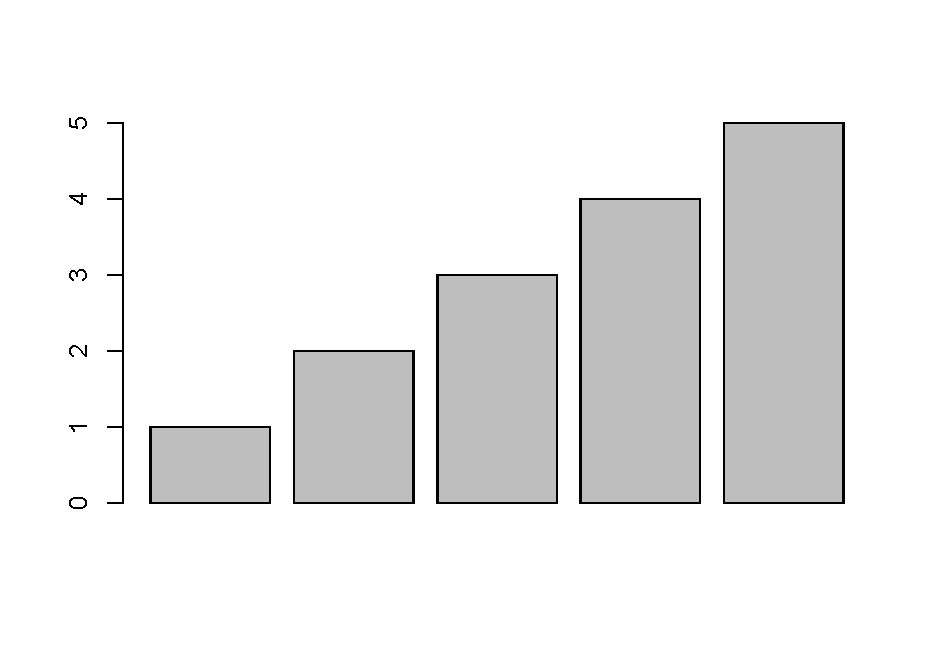
\includegraphics[width=0.8\hsize]{barplot01.pdf}
  \caption{これは図の例で、棒グラフが書かれている。}
  \label{fg:figure-example}
\end{figure}


最初の表の番号は「表\ref{tb:table-example}」である。

\begin{table}[h]
  \caption{これは表の例で、3行3列から成り立っている。}
  \label{tb:table-example}
  \begin{center}
    \begin{tabular}{lll} \toprule
      見出し1 & 見出し2 & 見出し3 \\ \midrule
      あああ & いいい & ううう \\
      かかか & ききき & くくく \\ \bottomrule
    \end{tabular}
  \end{center}
\end{table}

表\ref{tb:wide-table-example}は横長の表を90度回転したものである。

\begin{landscape}
  \begin{table}
    \caption{かなり横長の表の例。}
    \label{tb:wide-table-example}
    \begin{center}
      \begin{tabular}{lllllllllllll} \toprule
        言語名   & 月曜日     & 火曜日      & 水曜日       & 木曜日        & 金曜日       & 土曜日      & 日曜日      \\ \midrule
        ドイツ語  & Montag  & Dienstag & Mittwoch  & Donnerstag & Freitag   & Samstag  & Sonntag  \\
        フランス語 & lundi   & mardi    & mercredi  & jeudi      & vendredi  & samedi   & dimanche \\
        英語    & Monday  & Tuesday  & Wednesday & Thursday   & Friday    & Saturday & Sunday   \\
        スペイン語 & lunes   & martes   & miércoles & jueves     & viernes   & sábado   & domingo  \\ \bottomrule
      \end{tabular}
    \end{center}
  \end{table}
\end{landscape}

\section{囲み枠}

\begin{note}{囲み記事のタイトル}
囲み記事の文章がここに入る。
囲み記事の文章がここに入る。
囲み記事の文章がここに入る。
囲み記事の文章がここに入る。
囲み記事の文章がここに入る。
囲み記事の文章がここに入る。
囲み記事の文章がここに入る。
囲み記事の文章がここに入る。
\end{note}


\sanko{短い参考情報を提示するときのために使う。}

\begin{lstlisting}[caption=簡単なプログラムの例, label=ls:example]
x <- c(24, 23, 15, 52, 63)
mean(x) # 平均を計算
\end{lstlisting}


\section{特殊文字}

  \ajMaru{0} \ajMaru{5} \ajMaru{42} \ajMaru{100}
  \ajMaru*{0} \ajMaru*{5} \ajMaru*{42} \ajMaru*{100}
  \ajKuroMaru{0} \ajKuroMaru{5} \ajKuroMaru{42} \ajKuroMaru{100}
  \ajKuroMaru*{0} \ajKuroMaru*{5} \ajKuroMaru*{42} \ajKuroMaru*{100}

  \ajKaku{0} \ajKaku{5} \ajKaku{42} \ajKaku{100}
  \ajKaku*{0} \ajKaku*{5} \ajKaku*{42} \ajKaku*{100}
  \ajKuroKaku{0} \ajKuroKaku{5} \ajKuroKaku{42} \ajKuroKaku{100}
  \ajKuroKaku*{0} \ajKuroKaku*{5} \ajKuroKaku*{42} \ajKuroKaku*{100}

  \ajMaruKaku{0} \ajMaruKaku{5} \ajMaruKaku{42} \ajMaruKaku{100}
  \ajMaruKaku*{0} \ajMaruKaku*{5} \ajMaruKaku*{42} \ajMaruKaku*{100}
  \ajKuroMaruKaku{0} \ajKuroMaruKaku{5} \ajKuroMaruKaku{42} \ajKuroMaruKaku{100}
  \ajKuroMaruKaku*{0} \ajKuroMaruKaku*{5} \ajKuroMaruKaku*{42} \ajKuroMaruKaku*{100}


  \ajLig{○問} \ajLig{○答} \ajLig{○例} \ajLig{●問} \ajLig{●答} \ajLig{●例}

  \ajLig{□問} \ajLig{□答} \ajLig{□例} \ajLig{■問} \ajLig{■答} \ajLig{■例}

  \ajLig{◇問} \ajLig{◇答} \ajLig{◇例} \ajLig{◆問} \ajLig{◆答} \ajLig{◆例}

\backmatter
\printindex

\end{document}